\section{Introduction}
The BraTS scans are 3D volumes. The groups participating in the BraTS contest build neural networks that work with these volumes as input directly.

One of the groups participating on the contest is the Healthcare Imaging A.I. group of the medical faculty of the University of Bern. The constituent of this thesis
is Mauricio Reyes, who is also the head of this group.

Applying the Hausdorff distance mask method on the neural network developed by the group could be helpful to enhance the neural network.

\subsection{Docker setup}
\nblink{brats3D/01\_preprocess.ipynb}

All participants of the contest are required to provide Docker images containing their neural networks. The Docker containers have to conform to a specific format which
was specified by the contest organizers. This simplifies the evaluation of the neural network, because all neural networks can be used in the same fashion.

The Docker container can only analyze a single scan at a time. When analyzing multiple scans, the container has to be executed again.

The Docker daemon mounts a directory from the host system into the container. The directory should contain the input files (4 files in the NIFTI format, one for each modality). The container will write the result (volume segment of the tumor, also in the NIFTI format) into the same directory.

The execution time to analyze a single scan varies from container to container. For CPU based neural network, it takes between 3 to 6 minutes to analyze one scan. GPU based networks take around one to two minutes.

\subsection{Zero out cubes}
\nblink{brats3D/02\_generate\_slices.ipynb}
The 2D version of the algorithm works by removing information by drawing a black circle onto the image. In the 3D version, we remove a small cube from the input files.
We load the NIFTI file, set a cubic part of the loaded 3D matrix to zero and save the scan again. An example of a modified volume is shown in Figure \ref{brats3d_example}.

\begin{figure}[H]
\centering
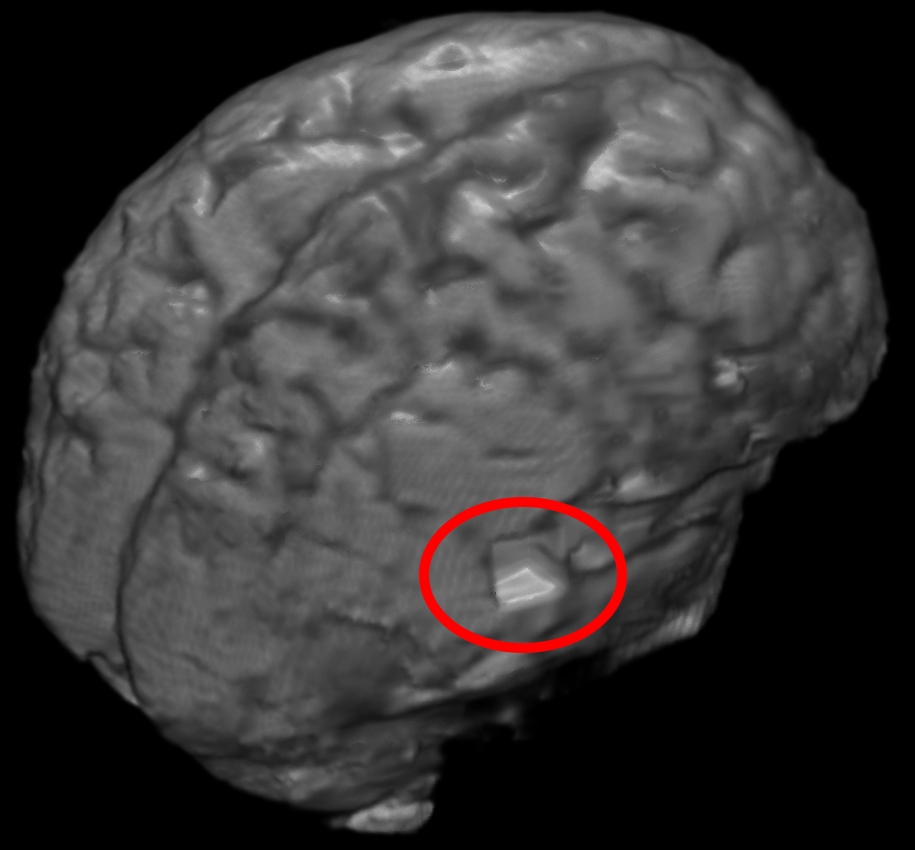
\includegraphics[width=8cm]{chapters/07_brats3d/images/brain-hdm-marked.png}
\caption{Modified scan with removed cube (red circle)}
\label{brats3d_example}
\end{figure}

\subsection{Docker execution}
\nblink{brats3D/03\_execute.ipynb}
To run the Docker container on all of our modified files, we have the correctly set up the directory that is mounte

\subsection{Distance calculation}
\nblink{brats3D/04\_calculate\_hausdorff\_distance.ipynb}
hausdorff + MSE

\subsection{Visualization}
We use cubes, do not bother with circles just upscale pixels

\subsection{Results}
\nblink{brats3D/02a\_generate\_single\_slice.ipynb}
\nblink{brats3D/06\_display\_single\_slice.ipynb}

\begin{figure}[H]
    \centering
    \begin{subfigure}{.33\textwidth}
        \centering
        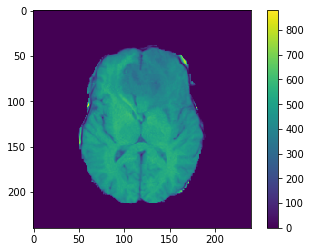
\includegraphics[width=\linewidth]{chapters/07_brats3d/images/01_t1.png}
        \caption{T1 modality of the slice}
    \end{subfigure}%
    \begin{subfigure}{.33\textwidth}
        \centering
        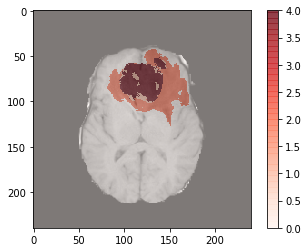
\includegraphics[width=\linewidth]{chapters/07_brats3d/images/05_t1_segment.png}
        \caption{T1 modality overlaid with ground truth tumor segment}
    \end{subfigure}
        \begin{subfigure}{.33\textwidth}
        \centering
        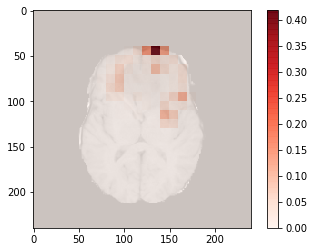
\includegraphics[width=\linewidth]{chapters/07_brats3d/images/09_t1_hdm10.png}
        \caption{T1 modality overlaid with hausdorff distance mask output}
    \end{subfigure}
    \caption{Visualization of the hausdorff distance mask result of the T1 modality. No big correlation between hausdorff distance mask output and actual tumor.}
\end{figure}

\begin{figure}[H]
    \centering
    \begin{subfigure}{.33\textwidth}
        \centering
        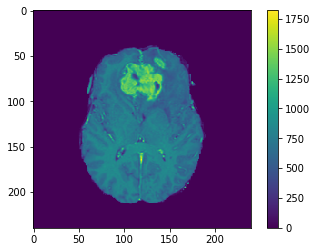
\includegraphics[width=\linewidth]{chapters/07_brats3d/images/02_t1ce.png}
        \caption{T1 contrast enhanced modality}
    \end{subfigure}%
    \begin{subfigure}{.33\textwidth}
        \centering
        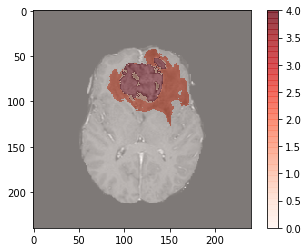
\includegraphics[width=\linewidth]{chapters/07_brats3d/images/06_t1ce_segment.png}
        \caption{T1 ce modality overlaid with ground truth tumor segment}
    \end{subfigure}
        \begin{subfigure}{.33\textwidth}
        \centering
        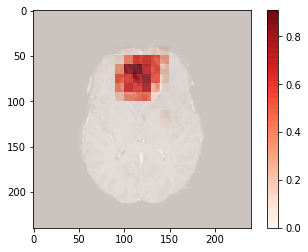
\includegraphics[width=\linewidth]{chapters/07_brats3d/images/10_t1ce_hdm.png}
        \caption{T1 ce modality overlaid with hausdorff distance mask output}
    \end{subfigure}
    \caption{Visualization of the hausdorff distance mask result of the T1 constract enhacned modality. Shows a correleation between the visible TODO}
\end{figure}


\begin{figure}[H]
    \centering
    \begin{subfigure}{.33\textwidth}
        \centering
        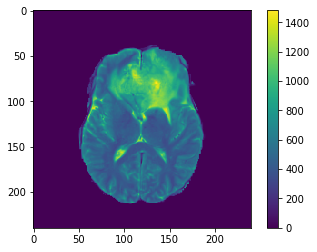
\includegraphics[width=\linewidth]{chapters/07_brats3d/images/03_t2.png}
        \caption{T2 modality of the slice}
    \end{subfigure}%
    \begin{subfigure}{.33\textwidth}
        \centering
        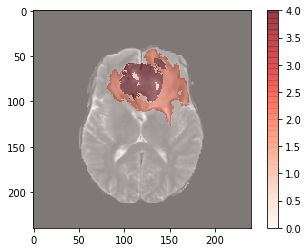
\includegraphics[width=\linewidth]{chapters/07_brats3d/images/07_t2_segment.png}
        \caption{T2 modality overlaid with ground truth tumor segment}
    \end{subfigure}
        \begin{subfigure}{.33\textwidth}
        \centering
        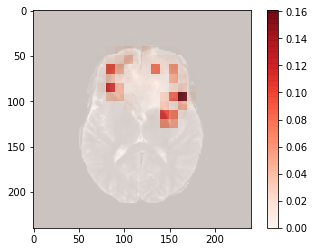
\includegraphics[width=\linewidth]{chapters/07_brats3d/images/11_t2_hdm.png}
        \caption{T2 modality overlaid with hausdorff distance mask output}
    \end{subfigure}
    \caption{T2}
\end{figure}

\begin{figure}[H]
    \centering
    \begin{subfigure}{.33\textwidth}
        \centering
        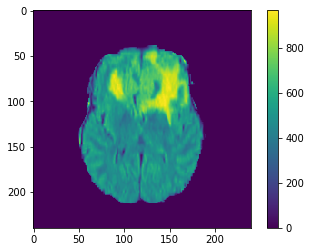
\includegraphics[width=\linewidth]{chapters/07_brats3d/images/04_flair.png}
        \caption{FLAIR modality of the slice}
    \end{subfigure}%
    \begin{subfigure}{.33\textwidth}
        \centering
        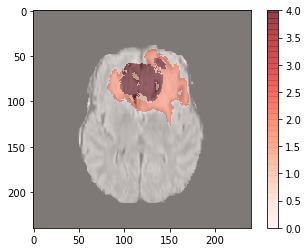
\includegraphics[width=\linewidth]{chapters/07_brats3d/images/08_flair_segment.png}
        \caption{FLAIR modality overlaid with ground truth tumor segment}
    \end{subfigure}
        \begin{subfigure}{.33\textwidth}
        \centering
        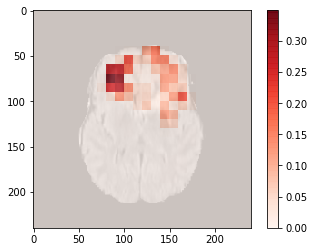
\includegraphics[width=\linewidth]{chapters/07_brats3d/images/12_flair_hdm.png}
        \caption{FLAIR modality overlaid with hausdorff distance mask output}
    \end{subfigure}
    \caption{Flair}
\end{figure}

\subsection{Discussion}


\subsection{Conclusion}
